\documentclass{article}


\usepackage[margin=1in]{geometry}
\usepackage{amsmath}
\usepackage{graphicx}
\usepackage{tabu}
\usepackage{color}
\usepackage{listings}
\usepackage{float}
\usepackage{caption}

\author{Zachary Vogel}
\title{Real Time Embedded Homework 2\\ ECEN 5623}
\date{\today}

\definecolor{codegreen}{rgb}{0,0.6,0}
\definecolor{codegray}{rgb}{0.5,0.5,0.5}
\definecolor{codepurple}{rgb}{0.58,0,0.82}
\definecolor{backcolour}{rgb}{0.95,0.95,0.92}
 
\lstdefinestyle{mystyle}{
    backgroundcolor=\color{backcolour},   
    commentstyle=\color{codegreen},
    keywordstyle=\color{magenta},
    numberstyle=\tiny\color{codegray},
    stringstyle=\color{codepurple},
    basicstyle=\footnotesize,
    breakatwhitespace=false,         
    breaklines=true,                 
    captionpos=b,                    
    keepspaces=true,                 
    numbers=left,                    
    numbersep=5pt,                  
    showspaces=false,                
    showstringspaces=false,
    showtabs=false,                  
    tabsize=2
}

\lstset{style=mystyle}

\begin{document}




\maketitle


\section*{Problem 1}
Implement a Linux process that is executed at the default priority for a user-level application and waits on a binary semaphore to be given by another application. Run this process and verify its state using the ps command to list its process descriptor. Now, run a separate process to give the semaphore causing the first process to continue execution and exit. Verify completion.\\

Here we see two screenshots proving my code does what it says it does. The actual code can be seen in the appendix.
\begin{figure}[H]
    \centering
    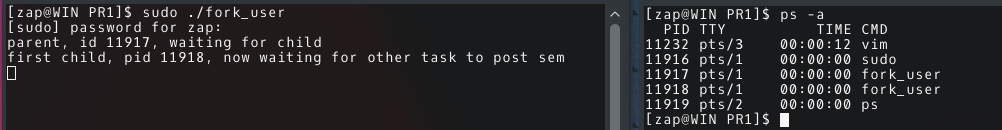
\includegraphics[width=\textwidth]{PR1/PR1_part1.png}
    \caption{As you can see, the process is waiting to finish}
\end{figure}
\begin{figure}[H]
    \centering
    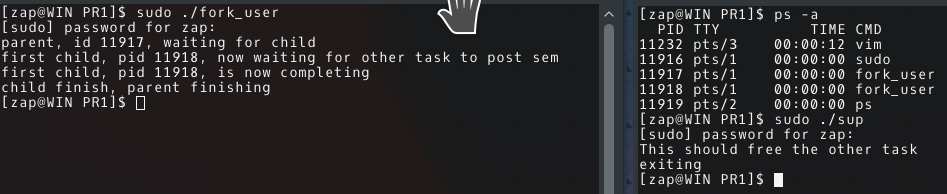
\includegraphics[width=\textwidth]{PR1/PR1_part2.png}
    \caption{Semaphore lock opened and everything finishes}
\end{figure}
\section*{Problem 2}
Why is the sufficient RM least upper bound so pessimistic?\\

The RM LUB is pessimistic largely because it is a sufficient not necessary condition. That means that the bound can't pass a set of tasks that won't be schedulable, but it can fail a task set that will be schedulable. The RM LUB is relatively easy to calculate, so it is better off being a simple sufficiency test as opposed to an extremelly complex necessary and sufficient test. The other reason for the pessimism is that task sets that aren't very harmonic will fail relatively easily
under a RM scheduling algorithm. That means that despite the high utilization of a harmonic task set under RM policy the bound must be lowered for the case where tasks aren't harmonic.


\section*{Problem 3}
If EDF can be shown to meet deadlines and potentially has 100\% CPU utilization, then why is it not typically the hard real-time policy of choice? That is, what are the drawbacks of using EDF compared to RM/DM? In an overload situation, how will EDF fail?\\

EDF scheduling has several major drawbacks that make it undesirable in real-time systems. First, EDF requires extra computation time because one must compute when the deadline happens and then restructure priorities based on that. The deadline time isn't always deterministic which can lead to problems and that extra computation can slow down the system. One will also notice that for lightly loaded systems EDF and RM scheduling often generate the exact same schedule for tasks. Similarly,
the more harmonic a systems tasks are the more likely that EDF and RM produce the same scheduling, so if one makes their tasks harmonic why not use the simpler RM policy. One more issue is that the sufficient bound for EDF scheduling is not easily computed as is the case for RM scheduling. It is also true that for harmonic task sets the RM policy can get an extremely high utilization. This is useful because tasks can often be made to be harmonic with minor adjustments to their
computation time.\\

The final reason that I found was in the case of a failing system. Rate monotonic scheduling guarantees that the highest priority task will be teh first task to miss a deadline if a deadline is going to be missed. This is very convenient for real time systems because of its determinism. Since one knows how the system will fail, they can build their system to react to that failure intelligently. This is not the case for EDF scheduling. In EDF scheduling, one does not know how a system will
fail. It might fail the highest period task or the lowest period task first. Since one does not know which task will fail it becomes much more difficult to "fail in an elegant way." Basically, EDF scheduling does not fail in a deterministic way, which makes it harder to work with in the case of failures and will often result in cascading failures. These result in many more missed deadlines which might end up breaking even a soft real time system.

\section*{Problem 4}
If a system must complete frame processing so that 100,000 frames are completed per second and the instruction count per frame processed is 2,120 instructions on a 1GHz processor core, what is the CPI required for the system? What is the overlap between instructions and IO time if the intermediate IO time is 4.5 $\mu$s?\\

For, $f=10^9$cycles/second, $IPF=2,120$instructions per frame, and $FPS=100,000$ frames per second, what is CPI. We need $2,120*100,000=212,000,000$ instructions per second. Then, CPI$=\frac{10^9}{212,000,000}=4.7169$CPI which is about 5 cycles per instruction. Given intermediate IO time is $4.5\mu$s, what is the overlap. The deadline time here is $10\mu$s because we want to complete 100,000 frames every second at even spacing. Instruction count time is the same based on the
definition of the system. Thus overlap percent is $1-\frac{10^{-5}-4.5*10^{-6}}{10^{-5}}=45\%$.

\section*{Problem 5}
Review the DVD code for heap\_mq.c and posix\_mq.c. Write a brief paragraph describing how the two message queue applications are similar and how they are different. Make sure you not only read the code but also build it, load it and execute it to make sure you understand how both applications work.\\

The first major difference between the two implementations is that heap\_mq.c creates and opens the message queue before running the sender and receiver functions. The posix\_mq.c code opens and creates the message queue in the receiver function and it is again opened in the sender function. The other major difference is that heap\_mq.c uses dynamically allocated memory to be used as the buffer, while posix\_mq.c uses stack memory. heap\_mq.c also implements the sender and receiver functions
as infinite loops that must be closed by deleting the tasks, while posix\_mq.c only runs through the sending and receiving once. Both functions give the receiver a higher priority than the sender, both use tasks to run the sender and receiver functions, and both use the posix queue with the function calls mq\_open, mq\_receive, and mq\_send.
\appendix
\section*{Code Appendix}
Waiting function at user priority
\lstinputlisting[language=C]{PR1/fork_user_prio.c}
Function to post the semaphore
\lstinputlisting[language=C]{PR1/sup.c}

\end{document}
